\documentclass[twoside]{book}

% Packages required by doxygen
\usepackage{fixltx2e}
\usepackage{calc}
\usepackage{doxygen}
\usepackage[export]{adjustbox} % also loads graphicx
\usepackage{graphicx}
\usepackage[utf8]{inputenc}
\usepackage{makeidx}
\usepackage{multicol}
\usepackage{multirow}
\PassOptionsToPackage{warn}{textcomp}
\usepackage{textcomp}
\usepackage[nointegrals]{wasysym}
\usepackage[table]{xcolor}

% Font selection
\usepackage[T1]{fontenc}
\usepackage[scaled=.90]{helvet}
\usepackage{courier}
\usepackage{amssymb}
\usepackage{sectsty}
\renewcommand{\familydefault}{\sfdefault}
\allsectionsfont{%
  \fontseries{bc}\selectfont%
  \color{darkgray}%
}
\renewcommand{\DoxyLabelFont}{%
  \fontseries{bc}\selectfont%
  \color{darkgray}%
}
\newcommand{\+}{\discretionary{\mbox{\scriptsize$\hookleftarrow$}}{}{}}

% Page & text layout
\usepackage{geometry}
\geometry{%
  a4paper,%
  top=2.5cm,%
  bottom=2.5cm,%
  left=2.5cm,%
  right=2.5cm%
}
\tolerance=750
\hfuzz=15pt
\hbadness=750
\setlength{\emergencystretch}{15pt}
\setlength{\parindent}{0cm}
\setlength{\parskip}{3ex plus 2ex minus 2ex}
\makeatletter
\renewcommand{\paragraph}{%
  \@startsection{paragraph}{4}{0ex}{-1.0ex}{1.0ex}{%
    \normalfont\normalsize\bfseries\SS@parafont%
  }%
}
\renewcommand{\subparagraph}{%
  \@startsection{subparagraph}{5}{0ex}{-1.0ex}{1.0ex}{%
    \normalfont\normalsize\bfseries\SS@subparafont%
  }%
}
\makeatother

% Headers & footers
\usepackage{fancyhdr}
\pagestyle{fancyplain}
\fancyhead[LE]{\fancyplain{}{\bfseries\thepage}}
\fancyhead[CE]{\fancyplain{}{}}
\fancyhead[RE]{\fancyplain{}{\bfseries\leftmark}}
\fancyhead[LO]{\fancyplain{}{\bfseries\rightmark}}
\fancyhead[CO]{\fancyplain{}{}}
\fancyhead[RO]{\fancyplain{}{\bfseries\thepage}}
\fancyfoot[LE]{\fancyplain{}{}}
\fancyfoot[CE]{\fancyplain{}{}}
\fancyfoot[RE]{\fancyplain{}{\bfseries\scriptsize Generated by Doxygen }}
\fancyfoot[LO]{\fancyplain{}{\bfseries\scriptsize Generated by Doxygen }}
\fancyfoot[CO]{\fancyplain{}{}}
\fancyfoot[RO]{\fancyplain{}{}}
\renewcommand{\footrulewidth}{0.4pt}
\renewcommand{\chaptermark}[1]{%
  \markboth{#1}{}%
}
\renewcommand{\sectionmark}[1]{%
  \markright{\thesection\ #1}%
}

% Indices & bibliography
\usepackage{natbib}
\usepackage[titles]{tocloft}
\setcounter{tocdepth}{3}
\setcounter{secnumdepth}{5}
\makeindex

% Hyperlinks (required, but should be loaded last)
\usepackage{ifpdf}
\ifpdf
  \usepackage[pdftex,pagebackref=true]{hyperref}
\else
  \usepackage[ps2pdf,pagebackref=true]{hyperref}
\fi
\hypersetup{%
  colorlinks=true,%
  linkcolor=blue,%
  citecolor=blue,%
  unicode%
}

% Custom commands
\newcommand{\clearemptydoublepage}{%
  \newpage{\pagestyle{empty}\cleardoublepage}%
}

\usepackage{caption}
\captionsetup{labelsep=space,justification=centering,font={bf},singlelinecheck=off,skip=4pt,position=top}

%===== C O N T E N T S =====

\begin{document}

% Titlepage & ToC
\hypersetup{pageanchor=false,
             bookmarksnumbered=true,
             pdfencoding=unicode
            }
\pagenumbering{roman}
\begin{titlepage}
\vspace*{7cm}
\begin{center}%
{\Large Proyecto 1 }\\
\vspace*{1cm}
{\large Generated by Doxygen 1.8.11}\\
\end{center}
\end{titlepage}
\clearemptydoublepage
\tableofcontents
\clearemptydoublepage
\pagenumbering{arabic}
\hypersetup{pageanchor=true}

%--- Begin generated contents ---
\chapter{Proyecto-\/1-\/estructuras}
\label{md_README}
\hypertarget{md_README}{}
Metodo de integración de Euler 
\chapter{Hierarchical Index}
\section{Class Hierarchy}
This inheritance list is sorted roughly, but not completely, alphabetically\+:\begin{DoxyCompactList}
\item \contentsline{section}{Euler\+Solver}{\pageref{classEulerSolver}}{}
\begin{DoxyCompactList}
\item \contentsline{section}{Linear\+Solver1}{\pageref{classLinearSolver1}}{}
\item \contentsline{section}{Linear\+Solver2}{\pageref{classLinearSolver2}}{}
\item \contentsline{section}{Linear\+Solver3}{\pageref{classLinearSolver3}}{}
\item \contentsline{section}{Linear\+Solver4}{\pageref{classLinearSolver4}}{}
\end{DoxyCompactList}
\end{DoxyCompactList}

\chapter{Class Index}
\section{Class List}
Here are the classes, structs, unions and interfaces with brief descriptions\+:\begin{DoxyCompactList}
\item\contentsline{section}{\hyperlink{classEulerSolver}{Euler\+Solver} }{\pageref{classEulerSolver}}{}
\item\contentsline{section}{\hyperlink{classLinearSolver1}{Linear\+Solver1} }{\pageref{classLinearSolver1}}{}
\item\contentsline{section}{\hyperlink{classLinearSolver2}{Linear\+Solver2} }{\pageref{classLinearSolver2}}{}
\item\contentsline{section}{\hyperlink{classLinearSolver3}{Linear\+Solver3} }{\pageref{classLinearSolver3}}{}
\item\contentsline{section}{\hyperlink{classLinearSolver4}{Linear\+Solver4} }{\pageref{classLinearSolver4}}{}
\end{DoxyCompactList}

\chapter{File Index}
\section{File List}
Here is a list of all documented files with brief descriptions\+:\begin{DoxyCompactList}
\item\contentsline{section}{include/{\bfseries Euler\+Solver.\+h} }{\pageref{EulerSolver_8h}}{}
\item\contentsline{section}{include/{\bfseries Linear\+Solver1.\+h} }{\pageref{LinearSolver1_8h}}{}
\item\contentsline{section}{include/{\bfseries Linear\+Solver2.\+h} }{\pageref{LinearSolver2_8h}}{}
\item\contentsline{section}{include/{\bfseries Linear\+Solver3.\+h} }{\pageref{LinearSolver3_8h}}{}
\item\contentsline{section}{include/{\bfseries Linear\+Solver4.\+h} }{\pageref{LinearSolver4_8h}}{}
\item\contentsline{section}{pruebas/\hyperlink{prueba__iteraciones_8cpp}{prueba\+\_\+iteraciones.\+cpp} }{\pageref{prueba__iteraciones_8cpp}}{}
\item\contentsline{section}{pruebas/\hyperlink{prueba__steps_8cpp}{prueba\+\_\+steps.\+cpp} }{\pageref{prueba__steps_8cpp}}{}
\end{DoxyCompactList}

\chapter{Class Documentation}
\hypertarget{classEulerSolver}{}\section{Euler\+Solver Class Reference}
\label{classEulerSolver}\index{Euler\+Solver@{Euler\+Solver}}


{\ttfamily \#include $<$Euler\+Solver.\+h$>$}



Inheritance diagram for Euler\+Solver\+:\nopagebreak
\begin{figure}[H]
\begin{center}
\leavevmode
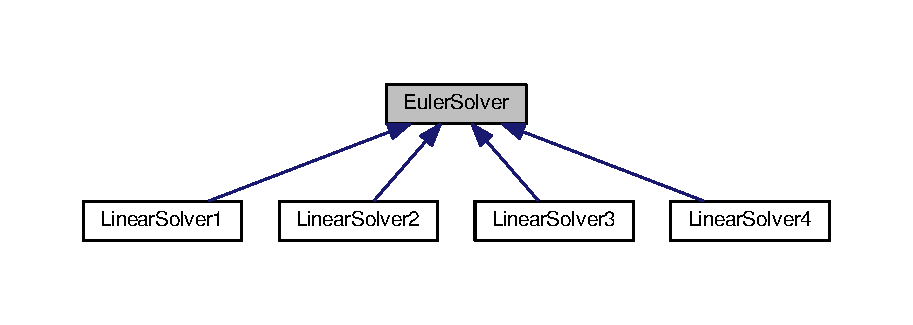
\includegraphics[width=350pt]{classEulerSolver__inherit__graph}
\end{center}
\end{figure}
\subsection*{Public Member Functions}
\begin{DoxyCompactItemize}
\item 
\hyperlink{classEulerSolver_a26e2d701b39e11176f147f7fe1d89e23}{Euler\+Solver} ()
\item 
virtual \hyperlink{classEulerSolver_ace90b1bc9a43703443e4caf7bf8f776d}{$\sim$\+Euler\+Solver} ()
\item 
void \hyperlink{classEulerSolver_af01d1179960dd710d670f4563633d12f}{set\+Initial\+Values} (double x0, double y0)
\item 
void \hyperlink{classEulerSolver_a58dbaa813c99143b7d1ba5c015135ed5}{set\+Step\+Size} (double h)
\item 
void \hyperlink{classEulerSolver_a85cb0e2f75a74a0999eeb5d5ca1a12e0}{set\+Integration\+Area} (double xf)
\item 
virtual double \hyperlink{classEulerSolver_ab9598d6adf761740607806988575ca0f}{Diff\+Equation} (double x, double y)=0
\item 
int \hyperlink{classEulerSolver_ab017374433f11690acb655a5d1d53a34}{solve} ()
\item 
int \hyperlink{classEulerSolver_aa7b5c95e6564dacb546833f3d8dd89d6}{get\+Data\+Values} (double $\ast$\&x, double $\ast$\&y, int \&size)
\end{DoxyCompactItemize}
\subsection*{Protected Member Functions}
\begin{DoxyCompactItemize}
\item 
void \hyperlink{classEulerSolver_af16a63dfc42f446e7fa312178707363d}{data\+Clear} ()
\end{DoxyCompactItemize}
\subsection*{Protected Attributes}
\begin{DoxyCompactItemize}
\item 
double {\bfseries h\+\_\+step}\hypertarget{classEulerSolver_a6bedf0a630f318074ade4745072260d4}{}\label{classEulerSolver_a6bedf0a630f318074ade4745072260d4}

\item 
double {\bfseries x\+\_\+initial}\hypertarget{classEulerSolver_ad2e74ab2d0c6ca0a85fe5e8abc45a71c}{}\label{classEulerSolver_ad2e74ab2d0c6ca0a85fe5e8abc45a71c}

\item 
double {\bfseries y\+\_\+initial}\hypertarget{classEulerSolver_aca7c9e78980015ca53b61db34c76e989}{}\label{classEulerSolver_aca7c9e78980015ca53b61db34c76e989}

\item 
double $\ast$ {\bfseries x\+\_\+data}\hypertarget{classEulerSolver_ae1b041e905fd619a42ca60125d7b8fb7}{}\label{classEulerSolver_ae1b041e905fd619a42ca60125d7b8fb7}

\item 
double $\ast$ {\bfseries y\+\_\+data}\hypertarget{classEulerSolver_a125cb8e3247bbb4cdbfdcf84b7164ed7}{}\label{classEulerSolver_a125cb8e3247bbb4cdbfdcf84b7164ed7}

\item 
int {\bfseries data\+\_\+size}\hypertarget{classEulerSolver_a4eef7bcc8af3b1ca05b197a6ef8d7739}{}\label{classEulerSolver_a4eef7bcc8af3b1ca05b197a6ef8d7739}

\end{DoxyCompactItemize}


\subsection{Detailed Description}
Clase abstracta para resolver ecuaciones diferenciales. 

\subsection{Constructor \& Destructor Documentation}
\index{Euler\+Solver@{Euler\+Solver}!Euler\+Solver@{Euler\+Solver}}
\index{Euler\+Solver@{Euler\+Solver}!Euler\+Solver@{Euler\+Solver}}
\subsubsection[{\texorpdfstring{Euler\+Solver()}{EulerSolver()}}]{\setlength{\rightskip}{0pt plus 5cm}Euler\+Solver\+::\+Euler\+Solver (
\begin{DoxyParamCaption}
{}
\end{DoxyParamCaption}
)\hspace{0.3cm}{\ttfamily [inline]}}\hypertarget{classEulerSolver_a26e2d701b39e11176f147f7fe1d89e23}{}\label{classEulerSolver_a26e2d701b39e11176f147f7fe1d89e23}
Constructor por defecto. \index{Euler\+Solver@{Euler\+Solver}!````~Euler\+Solver@{$\sim$\+Euler\+Solver}}
\index{````~Euler\+Solver@{$\sim$\+Euler\+Solver}!Euler\+Solver@{Euler\+Solver}}
\subsubsection[{\texorpdfstring{$\sim$\+Euler\+Solver()}{~EulerSolver()}}]{\setlength{\rightskip}{0pt plus 5cm}virtual Euler\+Solver\+::$\sim$\+Euler\+Solver (
\begin{DoxyParamCaption}
{}
\end{DoxyParamCaption}
)\hspace{0.3cm}{\ttfamily [inline]}, {\ttfamily [virtual]}}\hypertarget{classEulerSolver_ace90b1bc9a43703443e4caf7bf8f776d}{}\label{classEulerSolver_ace90b1bc9a43703443e4caf7bf8f776d}
Destructor por defecto. 

\subsection{Member Function Documentation}
\index{Euler\+Solver@{Euler\+Solver}!data\+Clear@{data\+Clear}}
\index{data\+Clear@{data\+Clear}!Euler\+Solver@{Euler\+Solver}}
\subsubsection[{\texorpdfstring{data\+Clear()}{dataClear()}}]{\setlength{\rightskip}{0pt plus 5cm}void Euler\+Solver\+::data\+Clear (
\begin{DoxyParamCaption}
{}
\end{DoxyParamCaption}
)\hspace{0.3cm}{\ttfamily [inline]}, {\ttfamily [protected]}}\hypertarget{classEulerSolver_af16a63dfc42f446e7fa312178707363d}{}\label{classEulerSolver_af16a63dfc42f446e7fa312178707363d}
Libera la memoria de los arreglos de datos X y Y. \index{Euler\+Solver@{Euler\+Solver}!Diff\+Equation@{Diff\+Equation}}
\index{Diff\+Equation@{Diff\+Equation}!Euler\+Solver@{Euler\+Solver}}
\subsubsection[{\texorpdfstring{Diff\+Equation(double x, double y)=0}{DiffEquation(double x, double y)=0}}]{\setlength{\rightskip}{0pt plus 5cm}virtual double Euler\+Solver\+::\+Diff\+Equation (
\begin{DoxyParamCaption}
\item[{double}]{x, }
\item[{double}]{y}
\end{DoxyParamCaption}
)\hspace{0.3cm}{\ttfamily [pure virtual]}}\hypertarget{classEulerSolver_ab9598d6adf761740607806988575ca0f}{}\label{classEulerSolver_ab9598d6adf761740607806988575ca0f}
Retorna el valor de la derivada. Define la ecuación de la primera derivada en función de X y Y es decir, f\textquotesingle{}(x,y). 
\begin{DoxyParams}{Parameters}
{\em x} & Valor de la variable x. \\
\hline
{\em y} & Valor de y. \\
\hline
\end{DoxyParams}
\begin{DoxyReturn}{Returns}
Resultado de la ecuación diferencial en el punto (x,y). 
\end{DoxyReturn}


Implemented in \hyperlink{classLinearSolver1_a9c05572054b1ab7f8974a7bb370a3f21}{Linear\+Solver1}, \hyperlink{classLinearSolver2_a23f2411fabb79e2d617cb4f89472be42}{Linear\+Solver2}, \hyperlink{classLinearSolver3_a120d9da579b9ba894079ac4a36b51280}{Linear\+Solver3}, and \hyperlink{classLinearSolver4_a75793f196b389479003e8ea6b9292af0}{Linear\+Solver4}.

\index{Euler\+Solver@{Euler\+Solver}!get\+Data\+Values@{get\+Data\+Values}}
\index{get\+Data\+Values@{get\+Data\+Values}!Euler\+Solver@{Euler\+Solver}}
\subsubsection[{\texorpdfstring{get\+Data\+Values(double $\ast$\&x, double $\ast$\&y, int \&size)}{getDataValues(double *&x, double *&y, int &size)}}]{\setlength{\rightskip}{0pt plus 5cm}int Euler\+Solver\+::get\+Data\+Values (
\begin{DoxyParamCaption}
\item[{double $\ast$\&}]{x, }
\item[{double $\ast$\&}]{y, }
\item[{int \&}]{size}
\end{DoxyParamCaption}
)\hspace{0.3cm}{\ttfamily [inline]}}\hypertarget{classEulerSolver_aa7b5c95e6564dacb546833f3d8dd89d6}{}\label{classEulerSolver_aa7b5c95e6564dacb546833f3d8dd89d6}
Copia por referencia los arreglos de datos x\+\_\+data, y\+\_\+data y el tamaño de los mismos. 
\begin{DoxyParams}{Parameters}
{\em x} & Puntero a los puntos en x. \\
\hline
{\em y} & Puntero a los puntos en y. \\
\hline
{\em size} & Tamaño de ambos arreglos de datos. \\
\hline
\end{DoxyParams}
\begin{DoxyReturn}{Returns}
NA 
\end{DoxyReturn}
\index{Euler\+Solver@{Euler\+Solver}!set\+Initial\+Values@{set\+Initial\+Values}}
\index{set\+Initial\+Values@{set\+Initial\+Values}!Euler\+Solver@{Euler\+Solver}}
\subsubsection[{\texorpdfstring{set\+Initial\+Values(double x0, double y0)}{setInitialValues(double x0, double y0)}}]{\setlength{\rightskip}{0pt plus 5cm}void Euler\+Solver\+::set\+Initial\+Values (
\begin{DoxyParamCaption}
\item[{double}]{x0, }
\item[{double}]{y0}
\end{DoxyParamCaption}
)\hspace{0.3cm}{\ttfamily [inline]}}\hypertarget{classEulerSolver_af01d1179960dd710d670f4563633d12f}{}\label{classEulerSolver_af01d1179960dd710d670f4563633d12f}
Define los valores iniciales. 
\begin{DoxyParams}{Parameters}
{\em x0} & Valor inicial en x. \\
\hline
{\em y0} & Valor de y(x0). \\
\hline
\end{DoxyParams}
\index{Euler\+Solver@{Euler\+Solver}!set\+Integration\+Area@{set\+Integration\+Area}}
\index{set\+Integration\+Area@{set\+Integration\+Area}!Euler\+Solver@{Euler\+Solver}}
\subsubsection[{\texorpdfstring{set\+Integration\+Area(double xf)}{setIntegrationArea(double xf)}}]{\setlength{\rightskip}{0pt plus 5cm}void Euler\+Solver\+::set\+Integration\+Area (
\begin{DoxyParamCaption}
\item[{double}]{xf}
\end{DoxyParamCaption}
)\hspace{0.3cm}{\ttfamily [inline]}}\hypertarget{classEulerSolver_a85cb0e2f75a74a0999eeb5d5ca1a12e0}{}\label{classEulerSolver_a85cb0e2f75a74a0999eeb5d5ca1a12e0}
Define el valor final. 
\begin{DoxyParams}{Parameters}
{\em xf} & Valor final. \\
\hline
\end{DoxyParams}
\index{Euler\+Solver@{Euler\+Solver}!set\+Step\+Size@{set\+Step\+Size}}
\index{set\+Step\+Size@{set\+Step\+Size}!Euler\+Solver@{Euler\+Solver}}
\subsubsection[{\texorpdfstring{set\+Step\+Size(double h)}{setStepSize(double h)}}]{\setlength{\rightskip}{0pt plus 5cm}void Euler\+Solver\+::set\+Step\+Size (
\begin{DoxyParamCaption}
\item[{double}]{h}
\end{DoxyParamCaption}
)\hspace{0.3cm}{\ttfamily [inline]}}\hypertarget{classEulerSolver_a58dbaa813c99143b7d1ba5c015135ed5}{}\label{classEulerSolver_a58dbaa813c99143b7d1ba5c015135ed5}
Define el paso de integración. 
\begin{DoxyParams}{Parameters}
{\em h} & Paso de integración. \\
\hline
\end{DoxyParams}
\index{Euler\+Solver@{Euler\+Solver}!solve@{solve}}
\index{solve@{solve}!Euler\+Solver@{Euler\+Solver}}
\subsubsection[{\texorpdfstring{solve()}{solve()}}]{\setlength{\rightskip}{0pt plus 5cm}int Euler\+Solver\+::solve (
\begin{DoxyParamCaption}
{}
\end{DoxyParamCaption}
)\hspace{0.3cm}{\ttfamily [inline]}}\hypertarget{classEulerSolver_ab017374433f11690acb655a5d1d53a34}{}\label{classEulerSolver_ab017374433f11690acb655a5d1d53a34}
Resuelve la ecuación diferencial para los parámetros dados. Obtiene los puntos (x,y) desde los valores iniciales (x0, y0), hasta el valor final de x, usando el paso de integración dado por h\+\_\+step. Los puntos se guardan en los arreglos x\+\_\+data y y\+\_\+data. 

The documentation for this class was generated from the following file\+:\begin{DoxyCompactItemize}
\item 
include/Euler\+Solver.\+h\end{DoxyCompactItemize}

\hypertarget{classLinearSolver1}{}\section{Linear\+Solver1 Class Reference}
\label{classLinearSolver1}\index{Linear\+Solver1@{Linear\+Solver1}}


Inheritance diagram for Linear\+Solver1\+:\nopagebreak
\begin{figure}[H]
\begin{center}
\leavevmode
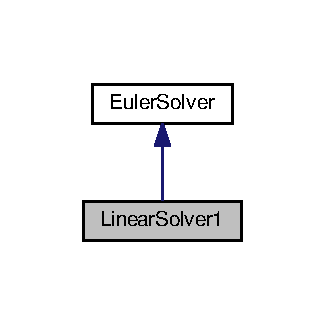
\includegraphics[width=156pt]{classLinearSolver1__inherit__graph}
\end{center}
\end{figure}


Collaboration diagram for Linear\+Solver1\+:\nopagebreak
\begin{figure}[H]
\begin{center}
\leavevmode
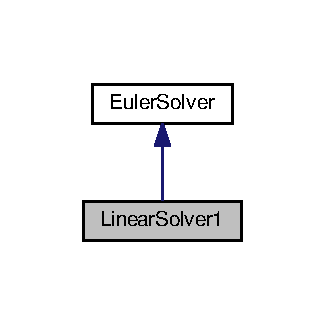
\includegraphics[width=156pt]{classLinearSolver1__coll__graph}
\end{center}
\end{figure}
\subsection*{Public Member Functions}
\begin{DoxyCompactItemize}
\item 
double \hyperlink{classLinearSolver1_a9c05572054b1ab7f8974a7bb370a3f21}{Diff\+Equation} (double x, double y)
\end{DoxyCompactItemize}
\subsection*{Additional Inherited Members}


\subsection{Member Function Documentation}
\index{Linear\+Solver1@{Linear\+Solver1}!Diff\+Equation@{Diff\+Equation}}
\index{Diff\+Equation@{Diff\+Equation}!Linear\+Solver1@{Linear\+Solver1}}
\subsubsection[{\texorpdfstring{Diff\+Equation(double x, double y)}{DiffEquation(double x, double y)}}]{\setlength{\rightskip}{0pt plus 5cm}double Linear\+Solver1\+::\+Diff\+Equation (
\begin{DoxyParamCaption}
\item[{double}]{x, }
\item[{double}]{y}
\end{DoxyParamCaption}
)\hspace{0.3cm}{\ttfamily [virtual]}}\hypertarget{classLinearSolver1_a9c05572054b1ab7f8974a7bb370a3f21}{}\label{classLinearSolver1_a9c05572054b1ab7f8974a7bb370a3f21}
Retorna el valor de la derivada. Define la ecuación de la primera derivada en función de X y Y es decir, f\textquotesingle{}(x,y). 
\begin{DoxyParams}{Parameters}
{\em x} & Valor de la variable x. \\
\hline
{\em y} & Valor de y. \\
\hline
\end{DoxyParams}
\begin{DoxyReturn}{Returns}
Resultado de la ecuación diferencial en el punto (x,y). 
\end{DoxyReturn}


Implements \hyperlink{classEulerSolver_ab9598d6adf761740607806988575ca0f}{Euler\+Solver}.



The documentation for this class was generated from the following files\+:\begin{DoxyCompactItemize}
\item 
include/Linear\+Solver1.\+h\item 
source/Linear\+Solver1.\+cpp\end{DoxyCompactItemize}

\hypertarget{classLinearSolver2}{}\section{Linear\+Solver2 Class Reference}
\label{classLinearSolver2}\index{Linear\+Solver2@{Linear\+Solver2}}


Inheritance diagram for Linear\+Solver2\+:\nopagebreak
\begin{figure}[H]
\begin{center}
\leavevmode
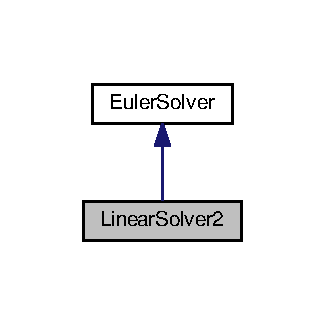
\includegraphics[width=156pt]{classLinearSolver2__inherit__graph}
\end{center}
\end{figure}


Collaboration diagram for Linear\+Solver2\+:\nopagebreak
\begin{figure}[H]
\begin{center}
\leavevmode
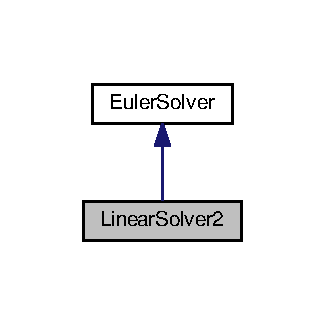
\includegraphics[width=156pt]{classLinearSolver2__coll__graph}
\end{center}
\end{figure}
\subsection*{Public Member Functions}
\begin{DoxyCompactItemize}
\item 
double \hyperlink{classLinearSolver2_a23f2411fabb79e2d617cb4f89472be42}{Diff\+Equation} (double x, double y)
\end{DoxyCompactItemize}
\subsection*{Additional Inherited Members}


\subsection{Member Function Documentation}
\index{Linear\+Solver2@{Linear\+Solver2}!Diff\+Equation@{Diff\+Equation}}
\index{Diff\+Equation@{Diff\+Equation}!Linear\+Solver2@{Linear\+Solver2}}
\subsubsection[{\texorpdfstring{Diff\+Equation(double x, double y)}{DiffEquation(double x, double y)}}]{\setlength{\rightskip}{0pt plus 5cm}double Linear\+Solver2\+::\+Diff\+Equation (
\begin{DoxyParamCaption}
\item[{double}]{x, }
\item[{double}]{y}
\end{DoxyParamCaption}
)\hspace{0.3cm}{\ttfamily [virtual]}}\hypertarget{classLinearSolver2_a23f2411fabb79e2d617cb4f89472be42}{}\label{classLinearSolver2_a23f2411fabb79e2d617cb4f89472be42}
Retorna el valor de la derivada. Define la ecuación de la primera derivada en función de X y Y es decir, f\textquotesingle{}(x,y). 
\begin{DoxyParams}{Parameters}
{\em x} & Valor de la variable x. \\
\hline
{\em y} & Valor de y. \\
\hline
\end{DoxyParams}
\begin{DoxyReturn}{Returns}
Resultado de la ecuación diferencial en el punto (x,y). 
\end{DoxyReturn}


Implements \hyperlink{classEulerSolver_ab9598d6adf761740607806988575ca0f}{Euler\+Solver}.



The documentation for this class was generated from the following files\+:\begin{DoxyCompactItemize}
\item 
include/Linear\+Solver2.\+h\item 
source/Linear\+Solver2.\+cpp\end{DoxyCompactItemize}

\hypertarget{classLinearSolver3}{}\section{Linear\+Solver3 Class Reference}
\label{classLinearSolver3}\index{Linear\+Solver3@{Linear\+Solver3}}


Inheritance diagram for Linear\+Solver3\+:\nopagebreak
\begin{figure}[H]
\begin{center}
\leavevmode
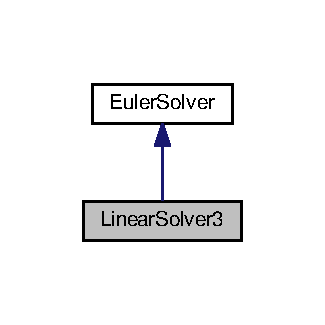
\includegraphics[width=156pt]{classLinearSolver3__inherit__graph}
\end{center}
\end{figure}


Collaboration diagram for Linear\+Solver3\+:\nopagebreak
\begin{figure}[H]
\begin{center}
\leavevmode
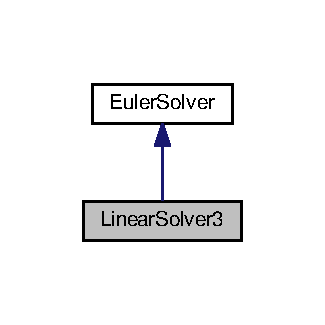
\includegraphics[width=156pt]{classLinearSolver3__coll__graph}
\end{center}
\end{figure}
\subsection*{Public Member Functions}
\begin{DoxyCompactItemize}
\item 
double \hyperlink{classLinearSolver3_a120d9da579b9ba894079ac4a36b51280}{Diff\+Equation} (double x, double y)
\end{DoxyCompactItemize}
\subsection*{Additional Inherited Members}


\subsection{Member Function Documentation}
\index{Linear\+Solver3@{Linear\+Solver3}!Diff\+Equation@{Diff\+Equation}}
\index{Diff\+Equation@{Diff\+Equation}!Linear\+Solver3@{Linear\+Solver3}}
\subsubsection[{\texorpdfstring{Diff\+Equation(double x, double y)}{DiffEquation(double x, double y)}}]{\setlength{\rightskip}{0pt plus 5cm}double Linear\+Solver3\+::\+Diff\+Equation (
\begin{DoxyParamCaption}
\item[{double}]{x, }
\item[{double}]{y}
\end{DoxyParamCaption}
)\hspace{0.3cm}{\ttfamily [virtual]}}\hypertarget{classLinearSolver3_a120d9da579b9ba894079ac4a36b51280}{}\label{classLinearSolver3_a120d9da579b9ba894079ac4a36b51280}
Retorna el valor de la derivada. Define la ecuación de la primera derivada en función de X y Y es decir, f\textquotesingle{}(x,y). 
\begin{DoxyParams}{Parameters}
{\em x} & Valor de la variable x. \\
\hline
{\em y} & Valor de y. \\
\hline
\end{DoxyParams}
\begin{DoxyReturn}{Returns}
Resultado de la ecuación diferencial en el punto (x,y). 
\end{DoxyReturn}


Implements \hyperlink{classEulerSolver_ab9598d6adf761740607806988575ca0f}{Euler\+Solver}.



The documentation for this class was generated from the following files\+:\begin{DoxyCompactItemize}
\item 
include/Linear\+Solver3.\+h\item 
source/Linear\+Solver3.\+cpp\end{DoxyCompactItemize}

\hypertarget{classLinearSolver4}{}\section{Linear\+Solver4 Class Reference}
\label{classLinearSolver4}\index{Linear\+Solver4@{Linear\+Solver4}}


Inheritance diagram for Linear\+Solver4\+:\nopagebreak
\begin{figure}[H]
\begin{center}
\leavevmode
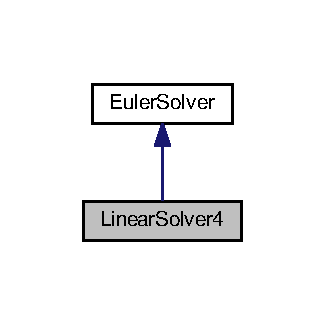
\includegraphics[width=156pt]{classLinearSolver4__inherit__graph}
\end{center}
\end{figure}


Collaboration diagram for Linear\+Solver4\+:\nopagebreak
\begin{figure}[H]
\begin{center}
\leavevmode
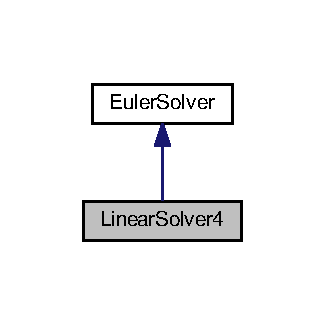
\includegraphics[width=156pt]{classLinearSolver4__coll__graph}
\end{center}
\end{figure}
\subsection*{Public Member Functions}
\begin{DoxyCompactItemize}
\item 
double \hyperlink{classLinearSolver4_a75793f196b389479003e8ea6b9292af0}{Diff\+Equation} (double x, double y)
\end{DoxyCompactItemize}
\subsection*{Additional Inherited Members}


\subsection{Member Function Documentation}
\index{Linear\+Solver4@{Linear\+Solver4}!Diff\+Equation@{Diff\+Equation}}
\index{Diff\+Equation@{Diff\+Equation}!Linear\+Solver4@{Linear\+Solver4}}
\subsubsection[{\texorpdfstring{Diff\+Equation(double x, double y)}{DiffEquation(double x, double y)}}]{\setlength{\rightskip}{0pt plus 5cm}double Linear\+Solver4\+::\+Diff\+Equation (
\begin{DoxyParamCaption}
\item[{double}]{x, }
\item[{double}]{y}
\end{DoxyParamCaption}
)\hspace{0.3cm}{\ttfamily [virtual]}}\hypertarget{classLinearSolver4_a75793f196b389479003e8ea6b9292af0}{}\label{classLinearSolver4_a75793f196b389479003e8ea6b9292af0}
Retorna el valor de la derivada. Define la ecuación de la primera derivada en función de X y Y es decir, f\textquotesingle{}(x,y). 
\begin{DoxyParams}{Parameters}
{\em x} & Valor de la variable x. \\
\hline
{\em y} & Valor de y. \\
\hline
\end{DoxyParams}
\begin{DoxyReturn}{Returns}
Resultado de la ecuación diferencial en el punto (x,y). 
\end{DoxyReturn}


Implements \hyperlink{classEulerSolver_ab9598d6adf761740607806988575ca0f}{Euler\+Solver}.



The documentation for this class was generated from the following files\+:\begin{DoxyCompactItemize}
\item 
include/Linear\+Solver4.\+h\item 
source/Linear\+Solver4.\+cpp\end{DoxyCompactItemize}

\chapter{File Documentation}
\hypertarget{prueba__iteraciones_8cpp}{}\section{pruebas/prueba\+\_\+iteraciones.cpp File Reference}
\label{prueba__iteraciones_8cpp}\index{pruebas/prueba\+\_\+iteraciones.\+cpp@{pruebas/prueba\+\_\+iteraciones.\+cpp}}
{\ttfamily \#include $<$iostream$>$}\\*
{\ttfamily \#include $<$Linear\+Solver1.\+h$>$}\\*
{\ttfamily \#include $<$Linear\+Solver2.\+h$>$}\\*
{\ttfamily \#include $<$Linear\+Solver3.\+h$>$}\\*
{\ttfamily \#include $<$Linear\+Solver4.\+h$>$}\\*
{\ttfamily \#include $<$Euler\+Solver.\+h$>$}\\*
{\ttfamily \#include $<$ctime$>$}\\*
{\ttfamily \#include $<$fstream$>$}\\*
{\ttfamily \#include $<$cstdlib$>$}\\*
Include dependency graph for prueba\+\_\+iteraciones.\+cpp\+:
\nopagebreak
\begin{figure}[H]
\begin{center}
\leavevmode
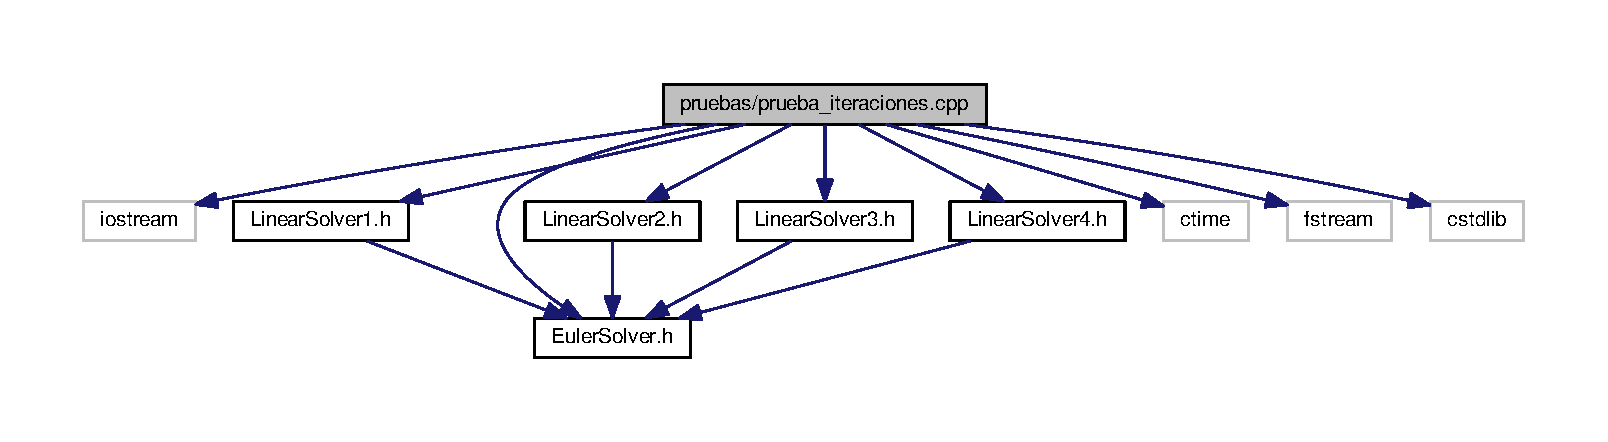
\includegraphics[width=350pt]{prueba__iteraciones_8cpp__incl}
\end{center}
\end{figure}
\subsection*{Functions}
\begin{DoxyCompactItemize}
\item 
int {\bfseries main} (int argc, char $\ast$argv\mbox{[}$\,$\mbox{]})\hypertarget{prueba__iteraciones_8cpp_a0ddf1224851353fc92bfbff6f499fa97}{}\label{prueba__iteraciones_8cpp_a0ddf1224851353fc92bfbff6f499fa97}

\end{DoxyCompactItemize}


\subsection{Detailed Description}
Prueba1. Recibe por linea de comandos\+: $<$num\+\_\+pruebas$>$ $<$prueba$>$ donde prueba es un numero entre 1 y 4. 
\hypertarget{prueba__steps_8cpp}{}\section{pruebas/prueba\+\_\+steps.cpp File Reference}
\label{prueba__steps_8cpp}\index{pruebas/prueba\+\_\+steps.\+cpp@{pruebas/prueba\+\_\+steps.\+cpp}}
{\ttfamily \#include $<$iostream$>$}\\*
{\ttfamily \#include $<$Linear\+Solver1.\+h$>$}\\*
{\ttfamily \#include $<$Linear\+Solver2.\+h$>$}\\*
{\ttfamily \#include $<$Linear\+Solver3.\+h$>$}\\*
{\ttfamily \#include $<$Linear\+Solver4.\+h$>$}\\*
{\ttfamily \#include $<$Euler\+Solver.\+h$>$}\\*
{\ttfamily \#include $<$ctime$>$}\\*
{\ttfamily \#include $<$fstream$>$}\\*
{\ttfamily \#include $<$cstdlib$>$}\\*
Include dependency graph for prueba\+\_\+steps.\+cpp\+:
\nopagebreak
\begin{figure}[H]
\begin{center}
\leavevmode
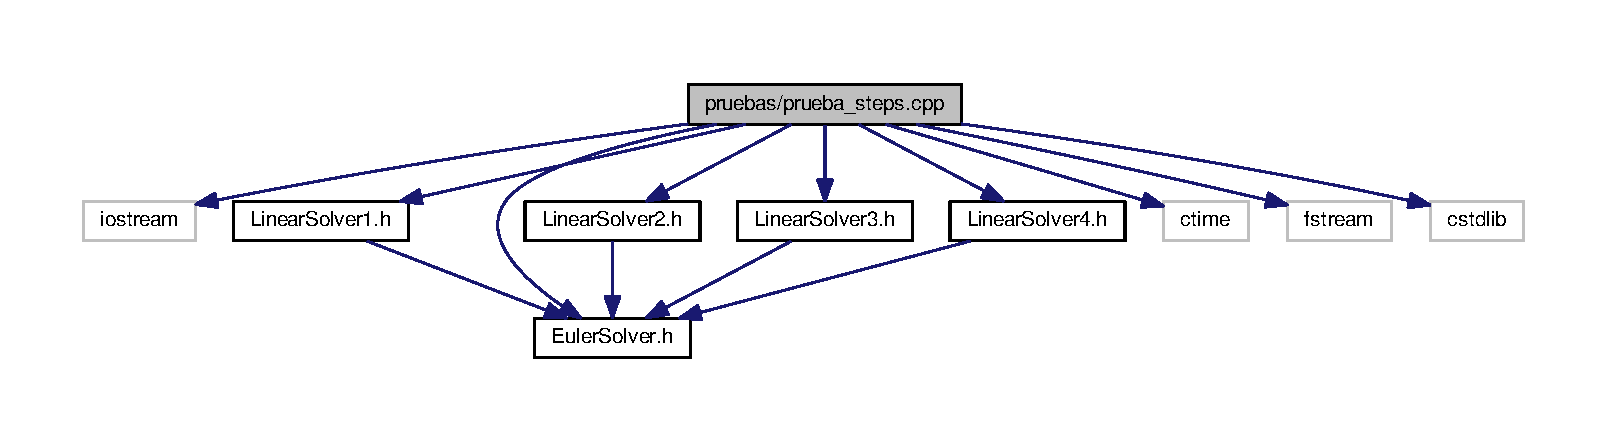
\includegraphics[width=350pt]{prueba__steps_8cpp__incl}
\end{center}
\end{figure}
\subsection*{Functions}
\begin{DoxyCompactItemize}
\item 
int {\bfseries main} (int argc, char $\ast$argv\mbox{[}$\,$\mbox{]})\hypertarget{prueba__steps_8cpp_a0ddf1224851353fc92bfbff6f499fa97}{}\label{prueba__steps_8cpp_a0ddf1224851353fc92bfbff6f499fa97}

\end{DoxyCompactItemize}


\subsection{Detailed Description}
Prueba2. Recibe por linea de comandos\+: $<$num\+\_\+pruebas$>$ $<$prueba$>$ donde prueba es un numero entre 1 y 4. 
%--- End generated contents ---

% Index
\backmatter
\newpage
\phantomsection
\clearemptydoublepage
\addcontentsline{toc}{chapter}{Index}
\printindex

\end{document}
